\documentclass[12pt,handout]{beamer}% version imprimable avec notes d’orateur, handout
\usepackage[couleur]{dipneuste}
\usepackage{pgfpages}
\uselanguage{French}
\languagepath{French}
%\usefonttheme[onlymath]{serif}
%\mode<beamer>{\usetheme{Darmstadt}%}
\setbeamercolor{math text}{fg=DarkBlue}%
\setbeamercolor{math text displayed}{fg=DarkBlue}
\setbeameroption{show only notes}

\title{Les colliers d'Antoine}
\author{Basile Pillet }
\date{Onzièmes journées Louis Antoine}

\newcommand<>{\pleinecran}[2]{{
    \setbeamertemplate{navigation symbols}{}
    \newgeometry{margin=0pt}
    \begin{frame}
    \includegraphics[width=\paperwidth]{#1}
    \note{#2}
    \end{frame}
    }
}
%\AtBeginSection{
    %\begin{frame}[c,plain,noframenumbering]
        %\tableofcontents[currentsection,hideothersubsections]
    %\end{frame}
%}

\newcommand\vis[1]{\fbox{\textcolor{DarkGreen}{#1}}}
\newcommand*{\vcenteredhbox}[1]{\begingroup
\setbox0=\hbox{#1}\parbox{\wd0}{\box0}\endgroup}


%\setbeamertemplate{note page}[plain]









\begin{document}

\begin{frame}
\maketitle
\begin{center}
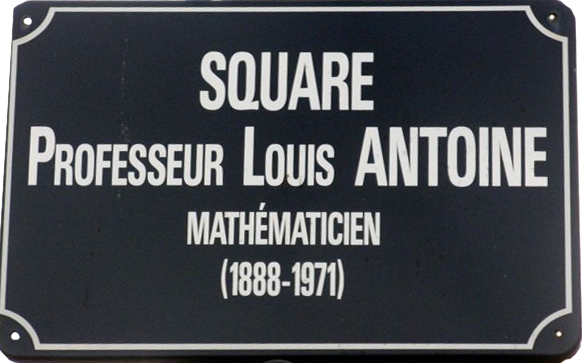
\includegraphics[scale=.2]{../Images/Square.png}
\end{center}
\end{frame}

\section{L'espace de Cantor}
\subsection{L'espace de Cantor intrins{\`e}que}
\subsubsection{L'ensemble}
\begin{frame}
\frametitle{On commence par $0$,}
\[
0
\]
\note{On commence par $0$,}
\end{frame}
\begin{frame}
\frametitle{puis on a $1$.}
\[
0 \quad 1
\]
\note{puis on a $1$.}
\end{frame}
\begin{frame}
\frametitle{On peut les combiner…}
\[
0 \quad 1
\]
\[
00 \quad 01 \quad 10 \quad 11
\]
\note{On voit ces objets comme des mots sur l'alphabet constitué des lettres $0$ et $1$. On peut s'en servir pour coder des entiers, des developpements décimaux, des signaux, des états d'un système simple à deux paramètres booléens indépendants.}
\end{frame}
\begin{frame}
\frametitle{… encore et encore…}
Mots de longueur $n$ sur l'alphabet $\{0,1\}$~:
\[
00\dots 0, \quad 00\dots 01, \quad \dots \quad 11 \dots 10, \quad 11 \dots 1
\]
\note{On voit ces objets comme des mots sur l'alphabet constitué des lettres $0$ et $1$. On peut s'en servir pour coder des entiers, des developpements décimaux, des signaux, des états d'un système simple…}
\pause
\[
\{0,1\}^n
\]
\note{On note $\{0,1\}^n$ cet ensemble}
\end{frame}
\begin{frame}
\frametitle{…jusqu'à l'infini !}
Mots infinis sur l'alphabet $\{0,1\}$~:
\[
011010011001011 \cdots
\]
\note[item]{On peut pousser la généralisation un peu plus loin et considérer des mots infinies de $0$ et $1$}
\pause
Suite $(u_n)_{n \in \N}$ avec $\forall i, u_i = 0$ ou $u_i = 1$. 
\note[item]{De manière rigoureuse, ce sont des suites (infinies)}
\pause
\[
\{0,1\}^\N \quad \text{ ou }\quad \{0,1\}^\omega
\]
\note[item]{On note leur ensemble $\{0,1\}^\N$}
\note[item]{Remarque : On vient déjà d'atteindre un niveau d'abstraction qui est inaccessible pour un ordinateur. Autant travailler avec des mots constitués de $0$ et de $1$ est très facile pour un ordinateur, autant considérer un objet infini ne lui est pas possible…}
\end{frame}
\begin{frame}
\frametitle{Ensemble de \textsc{Cantor}}
\[
C = \{0,1\}^\N
\]
\note{On appelle $C$ cet ensemble}
\end{frame}
\subsubsection{Cardinal}
\begin{frame}
\frametitle{Combien il y a-t-il d'éléments dans $C$ ?}
\pause
Une infinité :
\[
0 \ 0 \ 0 \ \cdots \underset{i\text{ ième position}}{0 \ \underbrace{1} \ 0\ 0\ } \cdots
\]
\note[item]{Les suites avec que des $0$ et un $1$ en $i$-ième position forment une infinité d'éléments différents de $C$. C'est une injection de $\N$ dans $C$.}
\pause
\begin{theorem}[G. Cantor, 1874]
L'ensemble $C$ n'est pas dénombrable.
\end{theorem}
\note[item]{En fait on a plus fort. Cet ensemble est strictement plus grand que $\N$.}
\note[item]{Historiquement, c'est comme ça que s'est dégagée la théorie des cardinaux.}
\end{frame}

\begin{frame}
\frametitle{Argument de Cantor}
\begin{center}\begin{tabular}{c|cccccc}
\hline 
 & $u_0$ & $u_1$ & $u_2$ & $u_3$ & $u_4$ & $\cdots$ \\ 
\hline 
0\; & 0 & 0 & 0 & 0 & 0 & $\cdots$ \\ 
1\; & 0 & 1 & 1 & 0 & 1 &$\cdots$ \\ 
2\; & 0 & 0 & 0 & 1 & 0 & $\cdots$ \\ 
3\; & 1 & 0 & 0 & 0 & 0 & $\cdots$ \\ 
4\; & 0 & 1 & 1 & 1 & 0 & $\cdots$ \\ 
5\; & 1 & 1 & 0 & 0 & 1 & $\cdots$ \\ 
\vdots &   &   &   &   &   &  \\ 
\hline 
\end{tabular}\end{center}
\bigskip
\note{Supposons que l'on ait une bijection entre $\N$ et $C$. Alors cette bijection peut se présenter sous forme de tableau comme cela.}
\end{frame}

\begin{frame}
\frametitle{Argument de Cantor}
\begin{center}\begin{tabular}{c|cccccc}
\hline 
 & $u_0$ & $u_1$ & $u_2$ & $u_3$ & $u_4$ & $\cdots$ \\ 
\hline 
0\; & \vis{0} & 0 & 0 & 0 & 0 & $\cdots$ \\ 
1\; & 0 & \vis{1} & 1 & 0 & 1 &$\cdots$ \\ 
2\; & 0 & 0 & \vis{0} & 1 & 0 & $\cdots$ \\ 
3\; & 1 & 0 & 0 & \vis{0} & 0 & $\cdots$ \\ 
4\; & 0 & 1 & 1 & 1 & \vis{0} & $\cdots$ \\ 
5\; & 1 & 1 & 0 & 0 & 1 & $\cdots$ \\ 
\vdots &   &   &   &   &   &  \\ 
\hline 
\end{tabular}\end{center}
\note[item]{Si on regarde la diagonale du tableau, on obtient une nouvelle suite de bits}
\pause
\[
\textcolor{DarkGreen}{0\; 1\; 0\; 0\; 0 \cdots}
\]
\pause
\note[item]{On peut alors considérer la suite "contraire" que l'on obtient en inversant chaque bit}
\[
1\; 0\; 1\; 1\; 1\; \cdots
\]
\note[item]{Cette nouvelle suite n'a alors pas sa place dans le tableau. En effet si elle etait rangé à la $k$-ième ligne, alors son $k$-ième bit serait celui de la diagonale (en vert) mais par définition ce serait aussi son contraire ! Impossible.}
\end{frame}
\begin{frame}
\begin{theorem}
$C$ est en bijection avec $\R$.
\end{theorem}
\pause
\bigskip
\textcolor{darkgray}{Corollaire du théorème de \textsc{Cantor-Bernstein}.}
\end{frame}

\subsubsection{Topologie}
\begin{frame}
\frametitle{Topologie}
\pause
\note[item]{On a defini un ensemble : l'ensemble des suites de 0 et de 1. On va maintenant s'autoriser à dire que deux suites sont "proches".}
\note[item]{"Deux suites sont d'autant plus proches qu'elles diffèrent loin."}
\[
0 0 0 0 0 0 0 0 0 0 0 0 0 0 0 0 0 0 0 0 0 0 0 …
\]
\[
0 0 0 0 0 0 0 0 0 0 0 0 0 0 0 0 0 0 0 0 0 \textcolor{DarkRed}{1} 0 …
\]
\pause
sont \textbf{plus proches} que 
\pause
\[
0 0 0 0 0 0 0 0 0 0 0 0 0 0 0 0 0 0 0 0 0 0 0 …
\]
\[
0 \textcolor{DarkRed}{1} 0 0 0 0 0 0 0 0 0 0 0 0 0 0 0 0 0 0 0 0 0 …
\]
\end{frame}

\begin{frame}
\begin{center}
\scalebox{5}{0} \; \scalebox{3.4}{1} \; \scalebox{2.25}{1} \; \scalebox{1.5}{0} \; 1 \; \scalebox{.7}{0}  \; \scalebox{.45}{0}  \; \scalebox{.3}{1} $\dots$ 
\end{center}
\end{frame}

\begin{frame}
\frametitle{Distance}
\note[item]{On donne la topologie via une distance, c'est-à-dire une mesure de la distance entre les points.}
\[
u,v \in C
\]

\[
d(u,v) = \sum_n \dfrac{|u_n-v_n|}{2^{n}}
\]
\pause
\begin{center}
$(C,d)$ est appelé \textbf{ l'espace de Cantor.}
\end{center}
\note[item]{On appelle cet espace métrique : "l'espace de Cantor" ou parfois simplement "Le Cantor"}
\end{frame}

\begin{frame}
\frametitle{Propriétés}
L'espace métrique $(C,d)$ est
\begin{enumerate}[<+->]
\item compact, \note[item]{COMPACT : \\(Tychonov) c'est la topologie produit et \{0,1\} est compact. Ou autrement, puisqu'on est métrique, il suffit de remarquer que toute suite de suite de bits admet une valeur d'adhérence qui est une suite des bits qui reviennent une infinité de fois (je sais pas si je dois le dire : faire une extraction diagonale à l'oral ça peut être technique).}
\item totalement discontinu (les composantes connexes sont des singletons), \note[item]{TOTALEMENT DISCONTINU :\\ On devrait plutôt totalement déconnecté, au sens où un point est toujours seul dans sa composante connexe.}
\item parfait (chaque point est dans l'adhérence de son complémentaire).\note[item]{PARFAIT : \\ Cependant chaque point est la limite d'une suite d'éléments de $C$ (distincts de lui)}
\end{enumerate}
\end{frame}

\begin{frame}
\frametitle{Caract{\'e}risation}
\begin{theorem}
Un espace métrisable non-vide est "le Cantor" \ssi il est~:
\begin{enumerate}[<+->]
\item compact,
\item totalement discontinu (les composantes connexes sont des singletons),
\item \only<3>{rigolo} \uncover<4->{parfait (chaque point est dans l'adhérence de son complémentaire).}
\end{enumerate}                                                
\end{theorem}
\note[item]{Un espace métrisable de même cardinal que $\R$ qui vérifie ces propriétés est homéomorphe à $C$}
\note[item]{Le fait qu'il est de même cardinal que $\R$ découle du théorème de Baire en utilisant compact (complet) et parfait : complet -> de Baire donc toute union dénombrable de fermés d'interieur vide est d'intérieur vide. Les singletons sont des fermés d'intérieur vide, donc si l'espace etait dénombrable, il serait d'intérieur vide, ce qui est absurde.}
\note[item]{Pour montrer que c'est un Cantor, il faut montrer qu'un tel espace admet une base dénombrable de voisinages ouverts et fermés. Découper l'espace en $2^n$ morceaux et construire par induction une app. vers $\{0,1\}^\N$.}
\end{frame}

\begin{frame}
\frametitle{Comparaison}
\note[item]{On a deux ensembles qui ont la même taille : $\R$ et $C$ et on veut les comparer.}
\note[item]{Pour comparer des espaces topologiques, on utilise les applications continues ; de la même manière que pour comparer les nombres on utilise des inégalités.}
\pause
\begin{block}{Question 1}
Quelles sont les applications continues $\R \longrightarrow C$ ?
\end{block}
\pause
\begin{exampleblock}{Réponse :} 
Que les constantes ! (coté totalement discontinu de $C$)
\end{exampleblock}
\pause
\begin{block}{Question 2}
Quelles sont les applications continues \only<5>{\textbf{injectives}} $C \longrightarrow \R$ \only<5>{qui soient un homéomorphisme sur leur image}?
\end{block}
\note[item]{Là par contre il va y en avoir beaucoup, on peut se concentrer uniquement sur celles qui ne perdent pas d'information (injectives). On les appelera par la suite "plongements".}
\end{frame}


\subsection{Les poussi{\`e}res de Cantor}

\subsubsection{Poussi{\`e}re lin{\'e}aire ou ensemble triadique de Cantor}
\begin{frame}% POUSSIERE DE CANTOR 1D
\begin{center}
\includegraphics<1>[scale=.4]{../Images/poussiere1D/1D1.pdf}
\includegraphics<2>[scale=.4]{../Images/poussiere1D/1D2.pdf}
\includegraphics<3>[scale=.4]{../Images/poussiere1D/1D3.pdf}
\includegraphics<4>[scale=.4]{../Images/poussiere1D/1D4.pdf}
\includegraphics<5>[scale=.4]{../Images/poussiere1D/1D5.pdf}
\includegraphics<6>[scale=.4]{../Images/poussiere1D/1D6.pdf}
\includegraphics<7>[scale=.4]{../Images/poussiere1D/1Df.pdf}
\end{center}
\note[item]{On part du segment $[0,1]$ que l'on a représenté en dessous épaissit}
\note[item]{On retire le tiers du milieu. On se retrouve donc avec l'union de deux segments}
\note[item]{On réitère le procédé avec chacun de ces 2 segments...}
\note[item]{etc...}
\note[item]{jusqu'à obtenir un espèce de code-barre ultrafin}
\note[item]{On remarque que si on zoomait sur ce qui était autrefois le premier tiers du segment de départ, on verrait un ensemble identique à ce qu'on a devant les yeux}
\note[item]{On dit que c'est un ensemble \emph{autosimilaire} ou fractale}
\end{frame}

\begin{frame}
\begin{center}
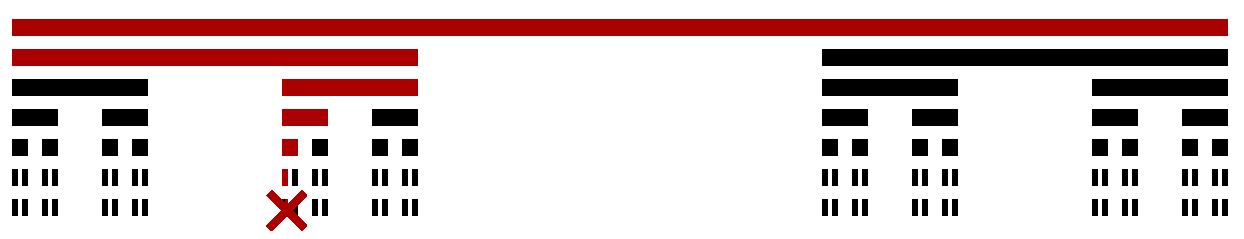
\includegraphics[scale=.4]{../Images/CantorParfait.pdf}
\end{center}
\note[item]{Ici on a une représentation des étapes de la construction. Un point de la poussière de Cantor linéaire est la donnée de la suite des segments qui le contiennent au cours de la construction.}
\pause
\begin{theorem}
L'ensemble construit est non-vide. Il est de plus 
\begin{itemize}[<+->]
\item compact, \note[item]{Suite décroissante de compacts}
\item totalement discontinu, \note[item]{Les composantes connexes à la $i$ième étape sont des segments de taille $3^{-i}$, à la limite, ce ne sont plus que des singletons}
\item parfait.\note[item]{Un point $x$ de la poussière est à l'étape $i$ dans un des petits segments. Soit $x_i$ un autre point de la poussière qui soit dans le même petit segment de l'étape $i$. On construit ainsi une suite d'éléments de la poussière, distincts de $x$ qui converge vers $x$.}
\end{itemize}
\pause
C'est un plongement de l'espace de Cantor dans $\R$.
\end{theorem}
\pause
L'espace construit est appelé \emph{poussière de Cantor triadique linéaire}.
\end{frame}

\subsubsection{Poussi{\`e}re plane}
\begin{frame}% POUSSIERE DE CANTOR 2D
\begin{center}
\includegraphics<1>[scale=1]{../Images/poussiere2D2/2D1.pdf}
\includegraphics<2>[scale=1]{../Images/poussiere2D2/2D2.pdf}
\includegraphics<3>[scale=1]{../Images/poussiere2D2/2D3.pdf}
\includegraphics<4>[scale=1]{../Images/poussiere2D2/2D4.pdf}
\includegraphics<5>[scale=1]{../Images/poussiere2D2/2D5.pdf}
\includegraphics<6>[scale=1]{../Images/poussiere2D2/2D6.pdf}
\includegraphics<7>[scale=1]{../Images/poussiere2D2/2Df.pdf}
\end{center}
\note[item]{On part du carré $[0,1]\times [0,1]$ dans le plan}
\note[item]{On retire le tiers vertical et le tiers horizontal du milieu. On se retrouve donc avec l'union de quatre carrés}
\note[item]{On réitère le procédé avec chacun de ces 2 segments...}
\note[item]{etc...}
\note[item]{C'est encore une fractale, au sens où si l'on zoomait sur le coin en haut à gauche, on retrouverait la même image}
\end{frame}

\begin{frame}
\begin{theorem}
L'ensemble construit est non-vide. Il est de plus 
\begin{itemize}
\item compact,
\item totalement discontinu,
\item parfait.
\end{itemize}
C'est un plongement de l'espace de Cantor dans $\R^2$.
\end{theorem}

\pause
L'espace construit est appelé \emph{poussière de Cantor triadique plane}.
\end{frame}


\subsubsection{Poussi{\`e}re spaciale}
\begin{frame}% POUSSIERE DE CANTOR 3D
\begin{center}
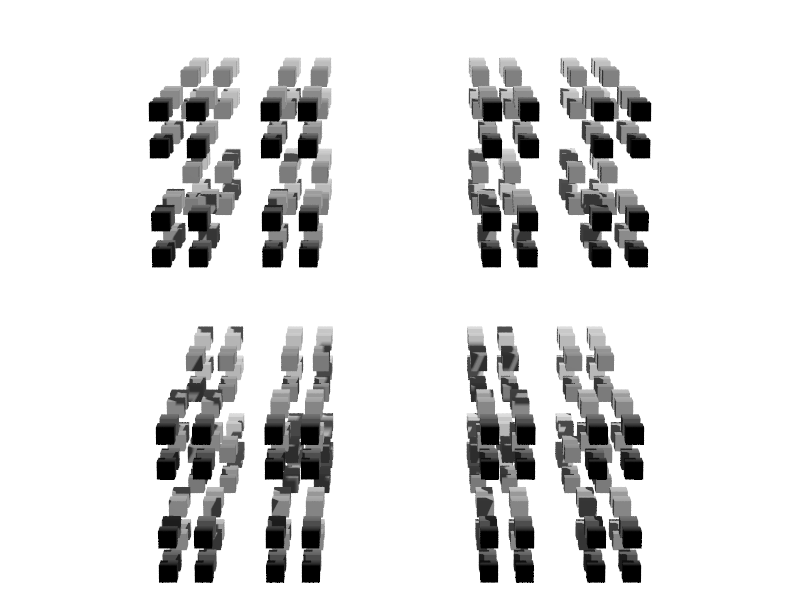
\includegraphics[scale=.35]{../Images/poussiere3D/Poussiere_Cantor_3D.png}
\end{center}
\note[item]{Ici à chaque étape je découpe mon cube par trois coups de couteau (vertical, horizontal et sur la profondeur), cette fractale ne doit pas être confondue avec l'éponge de Menger où le cube reste connexe à chaque étape (au lieu du couteau, c'est plus une fractale construite au tire-bouchon)}
\end{frame}

\pleinecran{../Images/Menger.png}{La poussière de Cantor spaciale ne doit pas être confondue avec l'éponge de Menger où le cube reste connexe à chaque étape (au lieu du couteau, c'est plus une fractale construite au tire-bouchon) (image wikipedia, auteur Niabot)}

\subsection{Le th{\'e}or{\`e}me de plongement équivalents}

\begin{frame}
\frametitle{Le cas du plan}
\pause
\begin{theorem}[Plongements équivalents]
Etant donnés deux poussières de Cantor dans $\R^2$, il existe un homéomorphisme de $\R^2$ qui les conjugue.
\end{theorem}
\note[item]{Théorème difficile (technique). Mais on peut le prouver sur un exemple}
\end{frame}

\begin{frame}% PREUVE
\begin{center}
\includegraphics<1>[scale=.1]{../Images/Theoreme/T0.pdf}
\includegraphics<2>[scale=.1]{../Images/Theoreme/T1.pdf}
\includegraphics<3>[scale=.1]{../Images/Theoreme/T2.pdf}
\includegraphics<4>[scale=.1]{../Images/Theoreme/T3.pdf}
\includegraphics<5>[scale=.1]{../Images/Theoreme/T4.pdf}
\includegraphics<6>[scale=.1]{../Images/Theoreme/T5.pdf}
\includegraphics<7>[scale=.1]{../Images/Theoreme/T6.pdf}
\includegraphics<8>[scale=.1]{../Images/Theoreme/T7.pdf}
\includegraphics<9>[scale=.1]{../Images/Theoreme/T8.pdf}
%\includegraphics<10>[scale=.15]{../Images/Theoreme/Tg.pdf}
\end{center}
\note[item]{On a deux copies du plan, l'une avec une poussière de Cantor linéaire sur l'axe des abscisse (en haut) et l'autre avec un poussière de Cantor plane}
\note[item]{On commence par construire un homéomorphisme du plan qui envoie le carré orange sur le rectangle orange (on peut même le faire par transformation affine)}
\note[item]{On considère les $4$ copies de notre poussière plane que l'on entoure par des carrés ouverts, et on regarde leurs images par l'homéomorphisme}
\note[item]{Mais quitte à modifier l'homéomorphisme sans toucher à ce qui est en dehors du rectange du haut, on peut ramener les taches jaunes sur des carrés centrés sur les $4$ copies de la poussière de cantor plane}
\note[item]{On est à nouveau dans la même situation que précédemment (vu que le carré en haut à gauche est similaire à la poussière plane dont on est parti) ; on peut donc réitérer le procédé.}
\note[item]{Le fait qu'on ait une suite d'homéomorphismes qui ne transforment qu'une partie de plus en plus petite du plan nous permet de passer à la limite et d'obtenir un homéomorphisme du plan qui conjugue les deux poussières}
\end{frame}

\begin{frame}
\begin{block}{Question}
Est-ce que c'est vrai dans $\R^3$ ?
\end{block}
\note[item]{Est-ce que si j'ai deux poussières de Cantor dans $\R^3$, il existe un homeomorphisme de $\R^3$ qui les conjugues ?}
\pause
\begin{center}
\vcenteredhbox{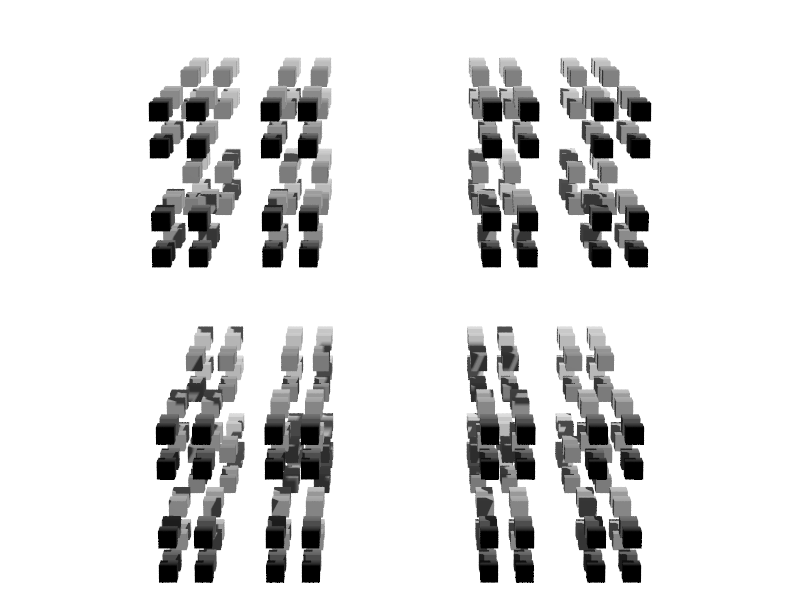
\includegraphics[scale=.15]{../Images/poussiere3D/Poussiere_Cantor_3D.png}} \quad
\vcenteredhbox{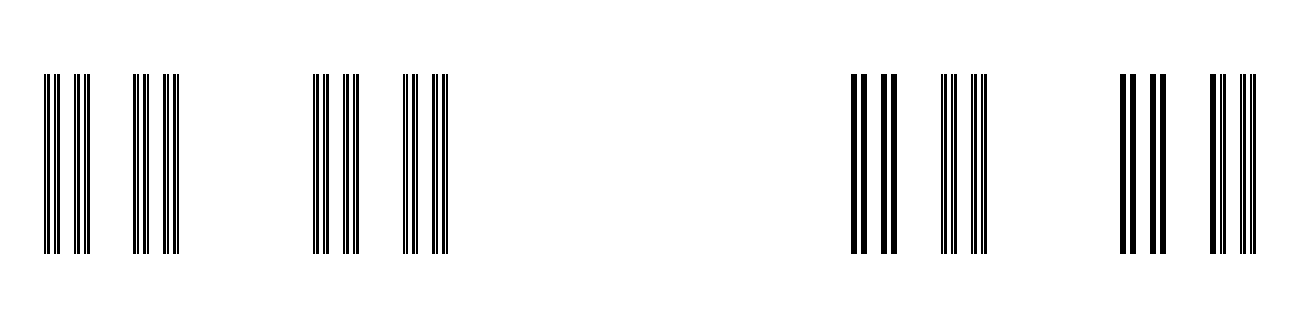
\includegraphics[scale=.15]{../Images/poussiere1D/1Df.pdf}}
\end{center}
\note[item]{Par le même raisonnement, on va pouvoir construire un homéo de $\R^3$ qui envoie ma poussière $3D$ sur la poussière $1D$}
\note[item]{On pourrait donc croire que ça va marcher pour toutes les plongements du Cantor dans $\R^3$…}
\end{frame}

\section{Louis Antoine}
\begin{frame}[c,plain,noframenumbering]%
        \tableofcontents[currentsection,hideothersubsections]
\end{frame}

\begin{frame}
\note[item]{…C'est là qu'arrive Louis Antoine. Tadaaaaaa !}
\begin{center}
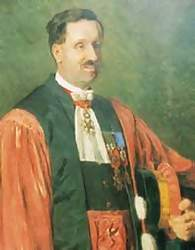
\includegraphics[scale=1]{../Images/Antoine2.jpg}
\end{center}
\note[item]{Louis Antoine né en 1888, se préparait à devenir professeur au Lycée, après de brillantes études à l'Ecole Normale Supérieure…}
\note[item]{…Quand la première guerre mondiale éclatat ! Mobilisé sur le front en Belgique, participe à la bataille de l'Yser (Il y a un boulevard à Rennes nommé d'après cette victoire), il est récompensé, nommé capitaine et chevalier de la legion d'honneur.}
\note[item]{La guerre continue, et c'est au printemps 1917, alors qu'il observait les positions ennemies à la jumelle, qu'il est blessé par obus qui lui ôte la vue…}
\end{frame}
\begin{frame}
\note[item]{La guerre se termine et il commence à s'inquiéter de son avenir : L'enseignement en lycée lui semble impossible. En discutant avec G. Julia et H. Lebesgue, ce dernier lui conseille de se tourner vers la recheche. Et pour éviter qu'il ait à se faire lire une bibliographie trop importante, Lebesgue l'oriente vers un domaine jeune à l'époque : la topologie (analysis situe) en basse dimension.}
\note[item]{ajoutant qu'il esperait que dans ce domaine "les yeux de l'esprit et l'habitude de la concentration remplaceront la vision perdue."}
\begin{center}
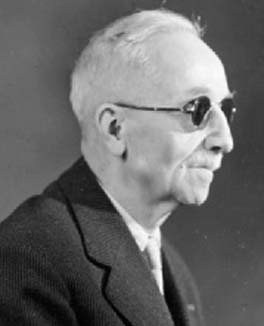
\includegraphics[scale=.75]{../Images/Antoine.jpg}
\end{center}
\note[item]{Louis Antoine soustient sa thèse à Strasbourg en 1921, où, comme on va le voir, il démontre le théorème précédent et réponds à la question qu'on vient de se poser en dimension $3$. Mais rapidement il devient professeur à Rennes 1925, et il parviendra à enseigner la géométrie, au tableau, malgrés les difficultés que l'on imagine…}
\note[item]{Se retire en 57, membre académie des sciences en 61 et meurs en 1971.}
\end{frame}

\section{Les colliers d'Antoine}
\begin{frame}[c,plain,noframenumbering]%
        \tableofcontents[currentsection,hideothersubsections]
\end{frame}

\subsection{Construction}
% COLLIER D'ANTOINE
\pleinecran{../Images/Iterations/1.png}{}%
\pleinecran{../Images/Iterations/2.png}{}%
\pleinecran{../Images/Iterations/3.png}{}%
\pleinecran{../Images/Iterations/4.png}{}%
\pleinecran{../Images/Iterations/5.png}{}%

\begin{frame}
\frametitle{Construction}
\begin{description}[<+->]
  \item[$V = C_0$] le tore plein du début (celui en vert),
  \item[$C_i$] la chaîne de tores plein à la $i$-ième étape,
  \item[$C_i^k$] Le $k$-ième tore de la chaîne à cette étape.
\end{description}
\pause
\[
A = \bigcap_{i \geq 0} C_i
\]\note[item]{$A$ est le collier d'Antoine spécifique à …}
\note[item]{Intersection décroissante des $C_i$}
\end{frame}

\begin{frame}
\frametitle{Un collier qui n'a que des perles…}
\begin{theorem}
\[A \cong C\]
\end{theorem}
\note[item]{Le collier d'Antoine est un plongement de $C$ dans $\R^3$}
\pause
Il suffit de vérifier~:
\begin{itemize}[<+->]
\item compact,
\item totalement discontinu,
\item parfait.
\end{itemize}
\note[item]{\textbf{compact} :
Intersection de compacts (union finies de tores)}
\note[item]{\textbf{totalement discontinu} (n'avoir que des perles) :
Si on prend un point du collier, c'est un point de notre chaîne de tores à l'étape $i$, or sa composante connexe à cette étape est un des tores $C_i^k$ dont le diamètre tend vers $0$ quand $i$ tend vers $+\infty$. (Pas rigoureux, mais convaiquant)}
\note[item]{\textbf{parfait} :
Je prends un point $x$ du collier. Et à chaque étape $i$ je prends un point $x_i$ qui est dans le même tore que $x$ mais distinct de $x$ (existe toujours car chaque tore est infini). Comme le diamètre des tores tends vers $0$, $x_i \rightarrow x$.}
\end{frame}

\subsection{Homotopie}

\begin{frame}
On appellera $P$ la poussière de Cantor triadique spaciale~:
\begin{center}
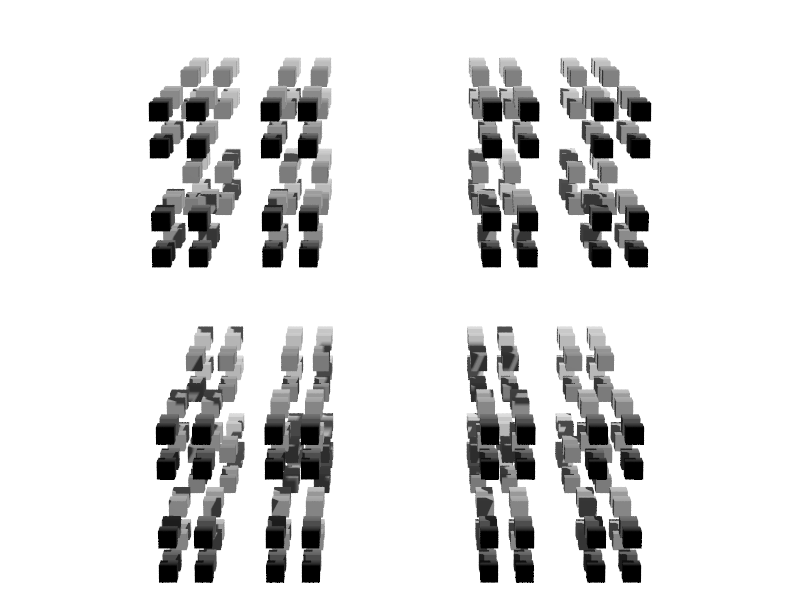
\includegraphics[scale=.2]{../Images/poussiere3D/Poussiere_Cantor_3D.png}
\end{center}
\end{frame}

\begin{frame}
\frametitle{… mais qui ne tombe pas !}
\begin{theorem}
Aucun des homéomorphismes $A \cong C \cong P$ ne se prolonge en un homeomorphisme de l'espace $\R^3$.
\end{theorem}
\pause
\begin{center}
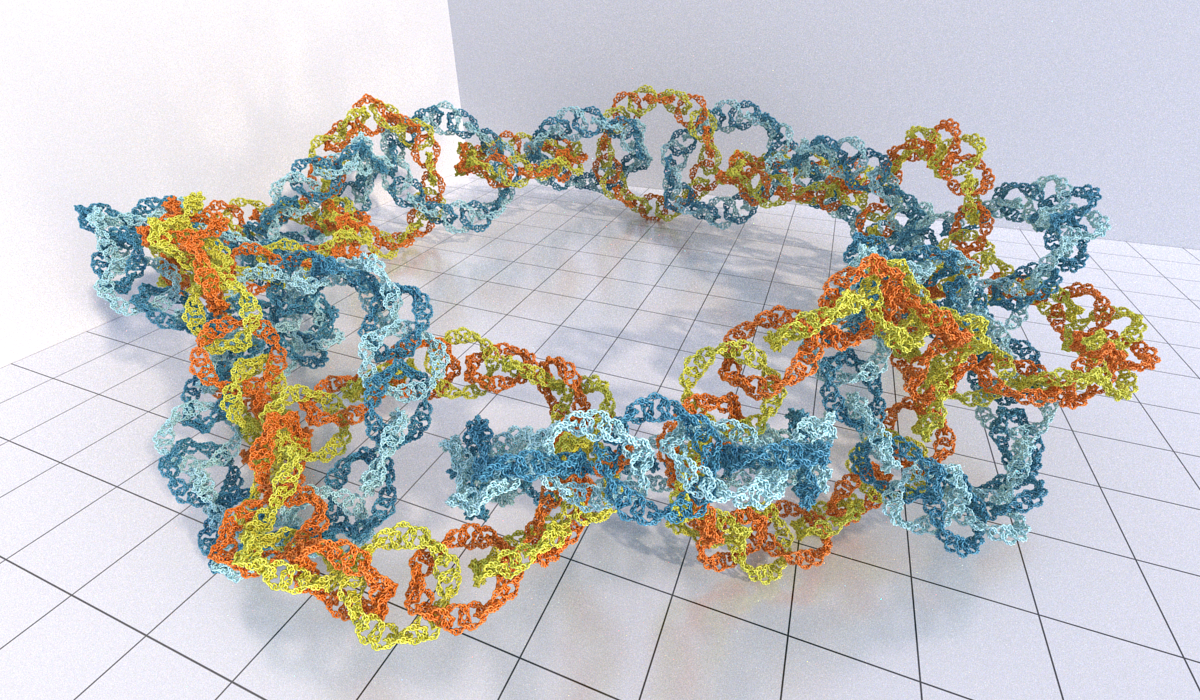
\includegraphics[scale=.15]{../Images/collier.png}
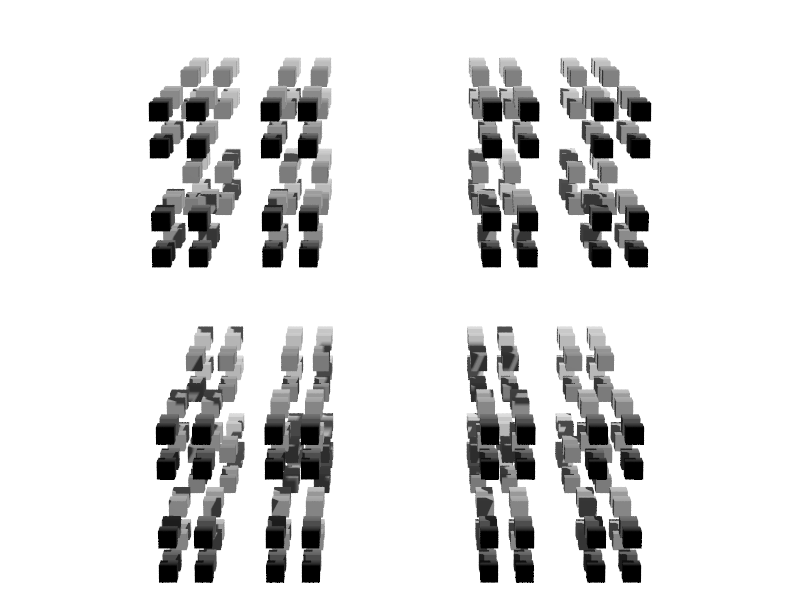
\includegraphics[scale=.15]{../Images/poussiere3D/Poussiere_Cantor_3D.png}
\end{center}
\note[item]{On va montrer que le collier, qui ne contient aucun lacet, aucune courbe, que des points ;  est pourtant "solide" au sens où il existe des lacets tracés dans son complémentaire qui ne se réduisent pas continuement en un point sans jamais intersecter le collier.}
\end{frame}

\begin{frame}
\frametitle{Réponse à la question dans $\R^3$}
\[\R^3\; \underset{\phi}{\tilde{\longrightarrow}}\; \R^3 , \; \phi(P) = A\]
\pause
\[\left(\R^3 \setminus P\right) \tilde{\longrightarrow} \left(\R^3 \setminus A\right)\]
\note[item]{Si on disposait d'un homéomorphisme $\R^3 \rightarrow \R^3$ qui envoie la poussière de Cantor classique sur le collier d'Antoine, alors…}
\note[item]{…Il induirait un homeomorphisme de leurs complémentaires}
\note[item]{…Mais dans le complémentaire du collier d'Antoine, le lacet ne peut se contracter, alors que dans le complémentaire de la poussière triadique, l'image du lacet est un lacet qui lui peut se contracter}
\end{frame}

\pleinecran{../Images/Iterations/homotopie.png}{Le lacet en noir ne peut pas se dénouer du collier. On peut montrer que même si le collier n'est plus qu'un ensemble de points, discontinu, le lacet ne peut pas se contracter en un point sans rencontrer le collier.}

\begin{frame}
\frametitle{Plongement sauvage}
\note[item]{En montrant que le lacet noir ne peut se contracter en un point, en fait on montre beaucoup plus fort :}
\note[item]{Le collier d'Antoine est un plongement de l'espace de Cantor dans $\R^3$ telle que le groupe fondamental de son complémentaire ne soit pas finiment engendré.}
\begin{theorem}
\begin{center}
$\pi_1(\R^3 \setminus A)$ n'est pas finiment engendré !
\end{center}
\end{theorem}
\end{frame}
\begin{frame}
On montre que
\[
\pi_1(\R^3 \setminus V) \uncover<2->{\varsubsetneq \pi_1(\R^3 \setminus C_1)} \uncover<3->{\varsubsetneq \pi_1(\R^3 \setminus C_2)} \uncover<4->{\varsubsetneq  \cdots} \uncover<5->{\varsubsetneq \pi_1(\R^3 \setminus A)}
\]
\note[item]{En fait le groupe fondamental du complémentaire du collier est la limite (au sens de "union") de tous ceux là.}
\end{frame}

\subsection{Infinité non dénombrable}
\begin{frame}
\frametitle{Différents colliers d'Antoine}
\pause
\note[item]{Le collier qui a été construit divise chaque tore en $24$ nouveau tores.}
\note[item]{Mais on aurait pu faire de même avec $2n$ nouveau tores. Et même en faisant varier le $n$ à chaque étape. Ou pour certains tores de certaines étapes.}
\begin{theorem}
Si deux colliers d'Antoine n'ont pas le même nombre de tores à une même étape de leur construction, alors ils sont \textbf{différents} \uncover<3->{(\textit{homéomorphes seulement en eux-mêmes})}.
\end{theorem}
\note[item]{Le théorème nous dit que pour différents choix, on obtiendra des colliers d'Antoine homéomorphe (des Cantor) mais dont les homéomorphismes ne se prolongent par à $\R^3$ tout entier.}
\note[item]{C'est le sens du mot \textbf{différents} : les plongements dans $\R^3$ ne sont pas conjugués par des homéos de $\R^3$. Antoine aurait dit "homéomorphes seulement en eux-mêmes".}
\pause
\pause
\begin{block}{Conséquence}
Il existe une infinité non-dénombrable de plongements $C \hookrightarrow \R^3$ \textbf{différents}.
\end{block}
\end{frame}

\section{Ouverture}
\begin{frame}[c,plain,noframenumbering]%
        \tableofcontents[currentsection,hideothersubsections]
\end{frame}

\begin{frame}
\begin{theorem}
\begin{itemize}[<+->]
\item[(Rappel)] Etant donnés deux poussières de Cantor dans $\R^2$, il existe un homéomorphisme de $\R^2$ qui les conjugue.
\item Etant donnés deux plongements de $\R$ dans $\R^2$ (courbes simples), il existe un homéomorphisme de $\R^2$ qui les conjugue.
\item Etant donnés deux plongements de $\S^1$ dans $\R^2$ (courbes simples fermées), il existe un homéomorphisme de $\R^2$ qui les conjugue.
\end{itemize}
\end{theorem}
\end{frame}

\begin{frame}
\frametitle{Et en dimension $3$}
\only<3>{\begin{center}
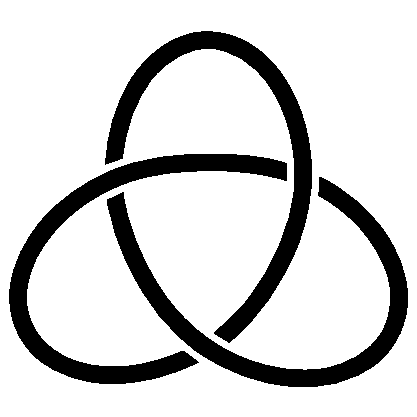
\includegraphics[scale=.5]{../Images/Trefle.pdf}
\end{center}}
\only<5>{\begin{center}
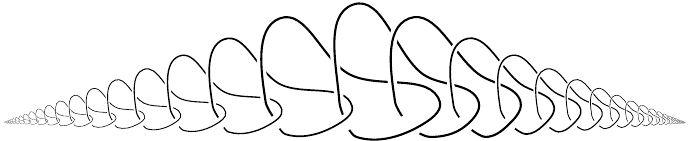
\includegraphics[scale=.5]{../Images/Fox-artin.png}
\end{center}}
\begin{itemize}
\item<1,2,4,6>[(Rappel)] Il existe des plongements \textbf{différents} de $C$ dans $\R^3$,
\item<2,4,6> il existe des plongements \textbf{différents} de $\S^1$ dans $\R^3$,
\item<4,6> {[(\textsc{Fox--Artin} 1948)]} il existe des plongements \textbf{différents} de $\R$ dans $\R^3$,
\item<6> {[(\name{J. W.}{Alexander} 1924)]} il existe des plongements \textbf{différents} de $\S^2$ dans $\R^3$.
\end{itemize}
\end{frame}

\begin{frame}
\begin{center}
\includegraphics<1>[scale=.4]{../Images/ASH/AHS_0.png}
\includegraphics<2>[scale=.4]{../Images/ASH/AHS_1.png}
\includegraphics<3>[scale=.5]{../Images/ASH/AHS_2.png}
\includegraphics<4>[scale=.5]{../Images/ASH/AHS_3.png}
\includegraphics<5>[scale=.5]{../Images/ASH/AHS_4.png}
%\includegraphics<6>[scale=.5]{../Images/ASH/AHS_5.png}
\end{center}
\note[item]{On part d'une sphère classique plongée dans $\R^3$ et on place à coté le tore qui est la première étape de notre construction du collier.}
\note[item]{On déforme la sphère juste dans un petit ouvert pour qu'elle vienne toucher le tore : on lui fait pousser une petite tentacule.}
\note[item]{On ne modifiera plus rien de la sphère en dehors de cet ouvert, on peut donc concentrer notre attention dessus.}
\note[item]{On passe à l'étape suivante de la construction du collier (ici avec 4 tores), et on fait pousser 4 sous-tentacules qui vont venir toucher chaquer des 4 tores, sans sortir du tore précédent.}
\note[item]{On réitère le procédé…}
\note[item]{Au final, on obtient toujours une sphère (il faut le montrer), mais son complémentaire dans $\R^3$ aura sa composante connexe non borné qui ne sera pas du tout simplement connexe !}
\end{frame}

\appendix

\bibliographystyle{amsalpha}
\nocite{*}
\begin{frame}
\bibliography{./Biblio.bib}
\end{frame}
\begin{frame}
\frametitle{Remerciements}
\begin{itemize}[<+->]
\item Merci à Arnaud Chéritat pour les images.
\item Merci aux organisateurs.
\item Merci de votre attention !
\end{itemize}
\end{frame}

\end{document}
